%%%%%%%%%%%%%%%%%%%%%%%%%%%%%%%%%%%%%%%%%%%%%%%%%
%% Part of Niles Johnson's latex setup
%% This document is in the public domain (2015)
%%%%%%%%%%%%%%%%%%%%%%%%%%%%%%%%%%%%%%%%%%%%%%%%%

\documentclass[11pt,oneside,draft]{amsart}
\usepackage{fouriernc} % Fourier fonts instead of Computer Modern

\usepackage{Environments}   % thm, prop, etc.
\usepackage{Definitions}    % macros
\usepackage{PageSetup}      % general setup


%%
%% Stuff for drafts only
%% 
\ifdraft{

%% uncomment to manually disable todonotes
%\PassOptionsToPackage{disable}{todonotes}

%% uncomment to manually disable watermark
%\PassOptionsToPackage{nostamp}{draftwatermark}

%% uncomment to manually disable label keys
%\PassOptionsToPackage{final}{showkeys}

%% watermark, todonotes, geometry
\usepackage{DraftSetup}

%% uncomment to restore default geometry 
%% defined in PageSetup
%\loadgeometry{default}

} % else (not draft)
{}





%%
%% Document-specific stuff
%%


%% document-specific options for hyperref
\hypersetup{
 pdfkeywords={latex starter,template},
 pdfauthor={Niles Johnson},
}



%% MSC
%% http://www.ams.org/mathscinet/msc/msc2010.html
\subjclass[2010]{68U15}

% 68U15 Text processing, mathematical typography
%
% 55P42 Stable homotopy theory, spectra
% 55N15 K-theory
% 18D10 Monoidal categories
% 18D05 Double categories, 2-categories, bicategories
% 19D23 Symmetric monoidal categories (in K-theory)
% 

\title[Latex package demo]{A Latex package demo\\ OR: What I've learned so far}

\address{Department of Mathematics,
The Ohio State University Newark}
\email{niles@math.osu.edu}
\urladdr{\url{http://nilesjohnson.net}}

\date{\today}

\begin{document}

\begin{abstract}
  This is a latex demo for moderate-to-advanced users of latex.  It illustrates
  some useful packages and habits I've developed over the years.  To
  really use it effectively, you probably have to eventually look at
  the separate documentation for each individual package.  Some of
  this is just a matter of taste (exceptionally good taste!) and some
  of this might seem like overkill now but become useful later.
\end{abstract}

\maketitle

\tableofcontents

\section{General comments}

This document uses 4 style files that I've developed for my texing.
I'll give an overview of the highlights in this document, but it's a
good idea to read through the included files and see what parts you do
and don't want to use.

The files are
\begin{itemize}
\item Environments: thm, prop, etc
\item PageSetup: stuff about page layout, references
\item Definitions: mostly macros
\item DraftSetup: stuff that's only for draft documents
\end{itemize}

First, here are some basic packages that are good to include
\begin{enumerate}
\item babel: language setting
\item fouriernc: font replacement including all math fonts, script and
  blackboard bold fonts.  Such font packages are exceedingly rare.
\item hyperref: linked references and better pdf documents
\item geometry: beter margin management
\item watermarkdraft: does what it says
\item showkeys: prints label keys in the margin
\end{enumerate}


\subsection{latexmk}\label{sec:latexmk}

This is a little script included with standard tex distributions.  It
checks file modification times and automatically runs latex as many
times as necessary, including bibtex if necessary.  It has a
continuous mode which watches files you're currently working on and
reruns on every update.

\subsection{text editor}

If you don't already have a good text editor, you should really start
using one.  You don't have to use all the features right away, but
over time you'll appreciate it more and more.  ``Good'' here means it
has the following, at minimum:
\begin{itemize}
\item tex or latex mode with syntax highlighting
\item support for automatically writing begin/end blocks
\item support for searching .bib file and inserting citation keys
\item support for finding and inserting appropriate label keys 
\item snippet support, for advanced macros
\item indentation and text re-flowing support.  60 charachters is a
  generally accepted guideline for good line length.
\end{itemize}
For these, I use emacs with RefTeX, AUCTeX, and yasnippet.  There are
many alternatives to match your taste. 

\subsection{version control}

This is beyond the scope of this document, but seriously look into
it.  It's \emph{such} a good idea.  I use git.

\subsection{\texorpdfstring{$\Gamma$}{Γ} and other tex in section headings}
If at all possible, avoid tex in section headings, because these are
put into the pdf table of contents, which can't process tex.  But if
you absolutely have to do it, use \verb|\texorpdfstring| and an
appropriate unicode alternative if you can find one.  Note that you
have to prerender unicode -- see \texttt{PageSetup.sty} 

\section{Cleveref}\label{sec:cleveref}

The cleveref package includes the environment name with the reference,
such as \cref{thm:atheorem}.  This is very useful for when you need to
change the environment type of a result.  It is clever about
referencing multiple results at once, such as
\cref{thm:atheorem,lem:btheorem,ctheorem,disp1,disp2}.

I generally prefix my labels with the environment type, to help keep
them straight in my mind, but this is unnecessary.

\begin{defn}  This is how to define a definition.
\end{defn}

And for a theorem and its proof you would type:

\begin{thm}\label{thm:atheorem}
This is the statement of a theorem.
\end{thm}
\begin{proof}
And this shows that the statement is correct.
\end{proof}

\begin{thm}\label{lem:btheorem}
  another theorem.  Try changing it to a lemma.
\end{thm}

\begin{thm}\label{ctheorem}
  a third theorem
\end{thm}

Here's an equation
\begin{equation}\label{disp1}
  e = mc^2
\end{equation}
This is the best environment to use for displayed diagrams too, so I
have cleveref just call the environment ``Display''.

For multiline equations, use ``\texttt{align}'' or
``\texttt{align*}'':

\begin{align}\label{disp2}
  (x + y)^2 & = (x+y) (x+y) \\
  & = x(x+y) + y(x+y) \nonumber\\
  & = x^2 + xy + yx + y^2 
\end{align}


\section{About text in tex}

\subsection{Symbols}

If you need the tex command for a symbol, the best way to get it
nowadays is
\href{http://detexify.kirelabs.org/classify.html}{Detexify}.

\subsection{fonts}

Develop a consistent system for how you use fonts.  I like to use Zapf
Chancery for named categories, such as $\Cat$, $\MonCat$, $\Ab$, etc.
Then I use Euler Cal for categories, such as $\cA$, $\cB$, $\cC$,
etc.  I use Ralph Smith Formal Script for fancy script, such as $\sA$,
$\sB$, $\sC$.


\subsection{Further comments on text}

If you want to \emph{emphasize} something in your text, use
\verb|\emph{}|.  For \textbf{boldface}, \textit{italics},
\texttt{monospace}, and \textsc{smallcaps}, use \verb|\textbf{}|
\verb|\textit{}|, \verb|\texttt{}|, and \verb|\textsc{}|.

These are modern improvements over the older \verb|\bf| etc.

\subsection{Punctuation}

Punctuation should go outside of math mode, otherwise the spacing will
be off.  As in $a$, $b$, and $c$.

Tex puts more space after sentence-ending punctuation, so if you use a
period mid-sentence, use the tilde to give a normal (and non-breaking)
space.  As in, e.g.~this sentence.

In math-mode, a hyphen is interpreted as a minus sign.  So if you want
to write $G\mh\Cat$ for the category of $G$ categories, you need to
use \verb|\mathrm{-}| or the macro \verb|\mh|.


\section{TikZ for more complex drawings}

TikZ is somewhat more full-featured than xypic.  It has an extensive
manual, a large online community, and a steep learning curve.  Here's one
example diagram:

\begin{center}
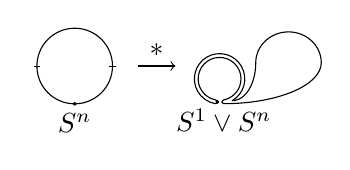
\begin{tikzpicture}[scale=.8]
  \draw (-2.5,-.05) node (t) {} 
  arc(-90:0:.6cm) node (h1) {}
  arc(0:180:.6cm) node (h2) {}
  arc(180:270:.6cm);
  \draw[fill=black] (t) circle (.02);
  \draw[very thin] (h1) ++(-.05,0) -- ++(.1,0);
  \draw[very thin] (h2) ++(-.05,0) -- ++(.1,0);

  \draw (t) ++(0,-.3cm) node {$S^n$};

  \draw[->] (t) ++(1cm,.6cm) -- node[above]{$*$}++(.6cm,0);
  \draw[cap=round,join=round] (0,0) 
  arc(-60:260:.4cm) 
  arc(-100:0:.03cm)
  node(x){}
  arc(0:80:.03cm)
  arc(260:-80:.34cm)
  arc(100:270:.03cm)
  arc(-90:0:1.55cm and .65cm)
  arc(0:180:.52cm and .49cm)
  arc(0:-85:.367cm and .602cm)
  --cycle;

  \draw[fill=black] (x) circle(.02);
  \draw (x) ++(.1cm,-.3cm) node{$S^1 \vee S^n$};
\end{tikzpicture}
\end{center}

\section{todonotes}
This is a package for adding \njnote{such as this} marginal notes in
your document.  For drafts.  Let's face it: for most of the time you
look at a tex document, it's a draft.
\njnoteil{you can also include inline notes}

\njmpar{such as this} 
And you can make marginal comments with no line.  See the package
documentation for more info (such as how to change the color, etc).

\section{Bibliography}

\njmpar{draft mode prints a black box to mark lines that latex could not
  break satisfactorily.  You have to reword them or do something else
  to handle them.  Usually best to ignore until the very final stages
  of editing.}
Here are some references to look at:  \cite{ATC,sage,JN2010Complex,GO2012Infinite,Eve1991Cohomology,Eve1961Cohomology,EKMM1997Rings,Ada1974Stable}

When you need new additions to your bibtex database, the best way to
get them is from \url{https://zbmath.org/} or
\url{http://www.ams.org/mathscinet/}.  Both give detailed citation
info in bibtex format for easy copy/pasting.  And both require a
subscription (i.e., a campus connection or proxy).  Zentralblatt has a
more forgiving search feature, and lets you see the first few matches
without subscription.  Often enough to get the database entries you need.

I use \href{http://jabref.sourceforge.net/}{JabRef} to manage my
database.  Although its interface is a little clunky, I like it for 4 reasons:
\begin{enumerate}
\item it automatically generates cite keys according to any pattern
  you like.  I use this pseudo-amsalpha pattern: \texttt{[authorsAlpha][year][veryshorttitle]}
\item you can add references by copy/pasting the bibtex source
\item it's cross-platform
\item it automatically alphabetizes your \texttt{.bib} file, which I
  like for those times I edit the file directly.
\end{enumerate}

This document uses a customization of the \texttt{amsalpha}
bibliography style.  It's additional features are:
\begin{enumerate}
\item First names of authors are always abbreviated.
\item The 'key' bibtex field is respected if present, and supercedes
  the author field, as in \cite{ATC,Sage}
\item The MR number is not printed, to avoid unfair promotion over
  Zentralblatt
\item The doi is printed if present, as in \cite{JN2010Complex}
\item A new arxiv field, as in \cite{GO2012Infinite,JN2010Complex}
\end{enumerate}
 

\section{Wait, there's more!}

Yes, really.  Typesetting is not at all a trivial art.  Just learn as
you go, and keep doing that.  There are other more extensive guides
for latex best-practices -- this document just represents what I've
been able to glean from them so far.

\section*{Acknowledgments}  

This document began as a template for REU students at the University
of Chicago.  Further improvements were made by Anna Marie Bohmann.
Niles Johnson made some other additions and modified it for a more
advanced audience.

\bibliographystyle{amsalpha2}
\bibliography{Refs}%


\end{document}

